\documentclass[journal]{IEEEtran}
\IEEEoverridecommandlockouts

%%%%%%%%%%%%%%%%%%%%%%%%%%%%%%%%%%%%%%
%%%%%%%% PACCHETTI PRINCIPALI %%%%%%%%
%%%%%%%%%%%%%%%%%%%%%%%%%%%%%%%%%%%%%%
\usepackage{fancyhdr}
\usepackage{graphicx}
\usepackage[italian]{babel}
\usepackage[utf8]{inputenc}
\usepackage{color}
\usepackage{hyperref}
\usepackage{wrapfig}
\usepackage{array}
\usepackage{multirow}
\usepackage{adjustbox}
\usepackage{nccmath}
\usepackage{subfigure}
\usepackage{amsfonts,latexsym}
\usepackage{enumerate}
\usepackage{booktabs}
\usepackage{float}
\usepackage{threeparttable}
\usepackage{array,colortbl}
\usepackage{ifpdf}
\usepackage{rotating}
\usepackage{cite}
\usepackage{stfloats}
\usepackage{url}
\usepackage{listings}
\usepackage{soul}

%%%%%%%%%%%%%%%%%%%%%%%%%%%%%%%%%%%%
%%% CREA E SCRIVI ALCUNI COMANDI %%%
%%%%%%%%%%%%%%%%%%%%%%%%%%%%%%%%%%%%
\newcolumntype{P}[1]{$>${\centering\arraybackslash}p{#1}}  %% Viene creato un nuovo tipo di colonna denominata P.

% correggere la sillabazione errata qui
\hyphenation{op-tical net-works semi-conduc-tor} %% Con questo comando si specifica come separare correttamente le sillabe nel caso in cui una parola si trovi in due diverse righe di testo

\graphicspath{ {img/} }  %%Percorso dove si trovano le immagini, se è vuoto indica che le immagini sono all'interno della stessa cartella che contiene il file .tex


%%%%%%%%%%%%%%%%%%%%%%%%%%%%%%%%%%%%%%%%%%%%%%%%
%%% INTESTAZIONE DELLE PAGINE TIPO UNICAFAM %%%%
%%%%%%%%%%%%%%%%%%%%%%%%%%%%%%%%%%%%%%%%%%%%%%%%
\newcommand{\MYhead}{\smash{\scriptsize
\hfil\parbox[t][\height][t]{\textwidth}{\centering
\begin{picture}(0,0) \put(-30,-13){
\includegraphics[width=30mm]{logoUnisalento.jpg}} \end{picture} \hspace{6.4cm}
INGEGNERIA INFORMATICA \\
\hspace{5.2cm} DIPARTIMENTO DI INGEGNERIA DELL'INNOVAZIONE \hspace{3cm} \\
\underline{\hspace{ \textwidth}}}\hfil\hbox{}}}
\makeatletter

% normal pages
\def\ps@headings{%
\def\@oddhead{\MYhead}%
\def\@evenhead{\MYhead}}%

% title page
\def\ps@IEEEtitlepagestyle{%
\def\@oddhead{\MYhead}%
\def\@evenhead{\MYhead}}%
\makeatother

% make changes take effect
\pagestyle{headings}

% adjust as needed
\addtolength{\footskip}{0\baselineskip}
\addtolength{\textheight}{-1\baselineskip}

%define colors for code language
\definecolor{codegreen}{rgb}{0,0.7,0.3}
\definecolor{codegray}{rgb}{0,0,0}
\definecolor{codepurple}{rgb}{0.58,0,0.82}
\definecolor{backcolour}{rgb}{0.95,0.95,0.95}
\definecolor{keywordcolor}{rgb}{0.8,0.3,0}

\lstdefinestyle{mystyle}{
    backgroundcolor=\color{backcolour},   
    commentstyle=\color{codegreen},
    keywordstyle=\color{keywordcolor},
    numberstyle=\tiny\color{codegray},
    stringstyle=\color{codepurple},
    basicstyle=\ttfamily\footnotesize,
    breakatwhitespace=false,         
    breaklines=true,                 
    captionpos=b,                    
    keepspaces=true,                 
    numbers=left,                    
    numbersep=5pt,                  
    showspaces=false,                
    showstringspaces=false,
    showtabs=false,                  
    tabsize=4
}

\lstset{style=mystyle}



%%%%%%%%%%%%%%%%%%%%%%%%%%%%%%%%
%%%%% INIZIO DEL DOCUMENTO %%%%%
%%%%%%%%%%%%%%%%%%%%%%%%%%%%%%%%
\begin{document}



%%%%%%%%%%%%%%%%%%%%%%%%%%%%
%%% TITOLO DEL DOCUMENTO %%%
%%%%%%%%%%%%%%%%%%%%%%%%%%%%
\title{Programmazione di Sistema e di Rete}



%%%%%%%%%%%%%%%%%%%%%%%%%%
%%%%%%%%% AUTORE %%%%%%%%%
%%%%%%%%%%%%%%%%%%%%%%%%%%
\author{Matteo Aprile\\
				Professore: Franco Tommasi\\
        }
        
%scrive il titolo
\maketitle

%scrive l'indice
\tableofcontents
\underline{\hspace{ 80 mm }}



%%%%%%%%%%%%%%%%%%%%%%%%%%%%%
%%% SEZIONI DEL DOCUMENTO %%%
%%%%%%%%%%%%%%%%%%%%%%%%%%%%%
\newpage
\section{Libri di testo consigliati}
\begin{itemize}
	\item Advanced Programming in the Unix Environment, 3th ed, Stevens, Rago
	\item TCP/IP 1, Stevens (facoltativo)
	\item Unix Networking Programming the Socket Networking API, Stevens
	\item The Linux Programing Interface, Kerrisk
	\item manset
	\item Gapil Guida alla Programmazione in Linux, Simone Piccardi
\end{itemize}
\newpage
\section{Comandi utili}

% find
\subsection{find: trovare tutti i file eseguibili}
	
\begin{lstlisting}
$ find . -type f -perm -0100
./standards/makeopt.awk
./standards/makeconf.awk
./proc/awkexample
./systype.sh
./advio/fixup.awk
\end{lstlisting}


\subsection{find: trovare file di intestazione del mac come stdio.h}

\begin{lstlisting}
find /Applications/Xcode.app/ -name stdio.h 2>/dev/null
\end{lstlisting}


% ldd
\subsection{lld: per capire che librerie usa il codice}

\begin{lstlisting}
ldd [nomevodice]
\end{lstlisting}


% gcc
\subsection{gcc: per vedere tutta la gerarchia di file in una libreria}

\begin{lstlisting}
gcc -H lib.a
\end{lstlisting}


\subsection{gcc: per vedere il codice con tutti i file importati}

\begin{lstlisting}
gcc -E file.c
\end{lstlisting}


\subsection{gcc -g: debugging debole}

\begin{lstlisting}
gcc -g -ansi -I../include -Wall -DMACOS -D_DARWIN_C_SOURCE  ls1.c -o ls1  -L../lib -lapue
\end{lstlisting}


\subsection{gcc -ggbd: debugging forte}

\begin{lstlisting}
gcc -ggbd -ansi -I../include -Wall -DMACOS -D_DARWIN_C_SOURCE  ls1.c -o ls1  -L../lib -lapue
\end{lstlisting}


% xattr
\subsection{xattr: usato per i file che entrano in quarantena su MacOS}

\begin{lstlisting}
xattr -d (delete) com.apple.quarantine [path sh]
\end{lstlisting}





\section{Variabili di sistema definite in .bashrc}

% INC
\subsection{INC}

\begin{lstlisting}
INC="/Applications/Xcode.app/Contents/Developer/Platforms/MacOSX.platform/Developer/SDKs/MacOSX.sdk/usr/include/"
\end{lstlisting}



\section{Introduzione - 23/27.09.22}

% System call
\subsection{System call}

Sono \hl{uguali alle funzioni di libreria dal punto di vista sintattico, pero' cambia il modo di compilarle}. Notare che non possono essere usati i nomi delle SC per delle function call.

Per poi poter "raccontare" tra umani le sequenze di bit che vengono mandate ai processori si usa \hl{assembly}.

Sono effettivamente delle chiamate a funzioni ma poi dal codice assembly puoi capire che è una system call dato che ha dei meccanismi specifici.

Alcuni esempi di chiamate e registri:
\begin{itemize}
	\item \textbf{eax} : registro dove metti il \textbf{numero della sc}
	\item \textbf{int 0x80}: \textbf{avvisa il kernel} che serve chiamare una sc
	\item \textbf{exit()}: chiudere un processo
	\item \textbf{write()}:
\end{itemize}

\begin{lstlisting}
mov edx,4    ; lunghezza messaggio
mov ecx,msg  ; puntatore al messaggio
mov ebx,1    ; file descriptor
mov eax,4    ; numero della sc
int 0x80	
\end{lstlisting}

dove nel \hl{file descriptor} indichi a quale file devi mandare l'output. Questo viene usato dato che così non deve cercare il path ogni volta ma lo mantiene aperto riferendosi ad esso tramite il numero.


% Programma Make
\subsection{Programma Make - 30.09.22}

Quando viene avviato verifica la presenza di un file chiamato "Makefile", oppure si usa 'make -f'. In questo file ci sono le \hl{regole di cosa fare per automatizzare delle azioni per un numero n di file}. Se, durante la compilazione di massa, \hl{una di queste da un errore il programma make si interrompe}, per evitare ciò si usa '-i' (ignore).

Il Makefile andrà ad aggiornare una libreria andando a guardare se una delle 3 date di ultima modifica si sono aggiornate.


Andiamo a guardare \hl{cosa contiene Makefile}:

\begin{lstlisting}
DIRS = lib intro sockets advio daemons datafiles db environ \
	fileio filedir ipc1 ipc2 proc pty relation signals standards \
	stdio termios threadctl threads printer exercises

all:
	for i in $(DIRS); do \
		(cd $$i && echo "making $$i" && $(MAKE) ) || exit 1; \
	done

clean:
	for i in $(DIRS); do \
		(cd $$i && echo "cleaning $$i" && $(MAKE) clean) || exit 1; \
	done
\end{lstlisting}

dove:
\begin{itemize}
	\item \hl{DIRS}: lo si associa alle \textbf{stringhe singole} che gli sono state associate
	\item \hl{all}: nel ciclo for:
		\begin{itemize}
			\item manda un comando in subshell
			\item \$\$i: riferimento alla variabile "i" del for + simbolo escape per il Makefile
			\item \$(MAKE): macro predefinita per i Makefile
		\end{itemize}
 
\end{itemize}

La struttura è:

\begin{lstlisting}
target: prerequisiti
	rule
\end{lstlisting}

dove:

\begin{itemize}
	\item \hl{target}: è l\textbf{a cosa che si vuole fare}, se essendo il primo target, sarà anche quello di default
	\item \hl{prerequisiti}: \textbf{file e/o target} a loro volta
	\item \hl{rule}: indica \textbf{cosa puo' fare il target}
\end{itemize}

Può capitare che prima di eseguire il Makefile ci sia uno \hl{script "configure"}. 

In molti casi si ha un \hl{target "clean"} che permette di pulire i file .o che sono inutili dopo la compilazione, o comunque qualsiasi tipo di file gli si voglia far eliminare. Questo tipo di target che non rappresentano un file, sono detti \hl{"phony"} perchè fasulli, dato che non sono file ma sole parole

\begin{lstlisting}
file: file.o lib.o

clean:
	rm file.o
\end{lstlisting}

Abbiamo delle \hl{variabili automatiche} per rendere il lavoro più facile:

\begin{itemize}
	\item \textbf{\$@}: per riferirsi il target
	\item \textbf{\$?}: tutti i prerequisiti più recenti del target
	\item \textbf{\$\^}: tutti i prerequisiti del target
	\item \textbf{\url{https://www.gnu.org/software/make/manual/make.html#Automatic-Variables}}
\end{itemize}


Un altro esempio di Makefile è:

\begin{lstlisting}
ROOT=..
PLATFORM=$(shell $(ROOT)/systype.sh)
include $(ROOT)/Make.defines.$(PLATFORM)

PROGS =	getcputc hello ls1 mycat shell1 shell2 testerror uidgid

all:	$(PROGS)

%:	%.c $(LIBAPUE)
	$(CC) $(CFLAGS) $@.c -o $@ $(LDFLAGS) $(LDLIBS)

clean:
	rm -f $(PROGS) $(TEMPFILES) *.o

include $(ROOT)/Make.libapue.inc
\end{lstlisting}

dove:

\begin{itemize}
	\item ROOT: cwd
	\item PLATFORM: assumera in valore del OS: macos/linux
	\item include: include un file
	\item PROGS: elenco dei programmi da usare
	\item \%: target con nome variabile, indica un file
	\item \%.c: target con nome variabile ma estensione .c
	\item \$(CC): indica il compilatore dove cc è un link simbolico a clang
	\item \$(CFLAGS) indica una macro predefinita dei default vuota che si può usare all'occorrenza
	\item all: target che prende in carico tutti i programmi che se saranno di tipo .c saranno presi in carico dal target successivo
\end{itemize}


\hl{Per la compilazione dei file}, qualsiasi sia il linguaggio, \hl{make saprà come compilarlo} grazie a tutte le definizioni di default presenti in:

\begin{lstlisting}
make -p
\end{lstlisting}

notare che \texdtbf{si può mettere un comando custom nelle rule} del target

Nell'eventualità di \hl{voler aggiornare un solo file della libreria senza far aggiornare il resto ci basterà usare uno script} che compila quel file passato a linea di comando.



% Direttive di preprocessore
\subsection{Direttive di preprocessore - 28.09.22}
Sono delle \hl{indicazioni date a gcc prima di iniziare la compilazione}.

Iniziano tutte con '\#':
\begin{itemize}
	\item \textbf{\#include}: serve ad \textbf{includere delle librerie} di sistema ($<$lib.h$>$) oppure di librerie fatte da noi e non in directory standard ("lib.h")
	\item \textbf{\#define}:
		\begin{itemize}
			\item permette di \textbf{creare delle "macro"}, che vanno a sostituire una stringa con un'altra (es: \#define BUFLEN), può capitare che debbano essere definite delle macro prima che si compili il programma, in questi casi si usa scrivere es: '-DMACOS'
			\item permette di \textbf{creare delle "function like macro"} (es: \#define ABSOLUTE\_VALUE(x) (((x$<$0)?-(x):(x))  
		\end{itemize}
		
	\item \textbf{\#ifdef, \#ifndef, \#endif}: usata per far accadere qualcosa nel caso un macro sia stata definita
\begin{lstlisting}
#ifdef VAR
print("hello");
#endif
\end{lstlisting}

\end{itemize} 

\hl{Per evitare che piu' file includano lo stesso si usano degli \#ifndef} in tutto il codice, in modo da evitare doppie definizioni.


% Librerie
\subsection{Librerie}

Durante la fase di compilazione creiamo dei file oggetto (.o) per ogni file in cui è scritta la descrizione delle funzioni di libreria (.c)

\begin{lstlisting}
gcc -c bill.c
\end{lstlisting}

Si andrà poi a creare il \hl{prototipo della funzione (.h)}.

In fine \hl{tramite il linker si andranno ad unire tutti i file per crearne uno unico} con tutte le definizioni delle funzioni incluse nelle librerie, di sistema e non, importate. Si vanno quindi a \hl{sciogliere tutti i riferimenti incrociati}.

\begin{lstlisting}
	gcc -o program program.o bill.o
\end{lstlisting}

Per quanto riguarda le \hl{funzioni di sistema} NON abbiamo il file sorgente ma abbiamo direttamente l'eseguibile. In compenso abbiamo un \hl{file di libreria}, cioè un insieme di file oggetto linkati in un unico file, dove c'è il codice oggetto di tutte le funzioni.

Abbiamo \textbf{2 tipi di librerie}:
\begin{itemize}
	\item \hl{statiche}: è una \textbf{collezione di file oggetto} che hanno il codice compilato delle funzioni e che verranno \textbf{linkati al momento della compilazione}. Il programma che si crea sarà possibile essere eseguito solo sullo stesso OS.
		
		Il \textbf{problema si ha nell'aggiornamento delle librerie al momento della scoperta di un bug}. Una volta coretto servirà ricevere la versione corretta per poter aggiornare il programma.
		
	\item \hl{dynamic}: ricordano il concetto di plug-in, quindi \textbf{viene invocato a runtime e caricato in memoria} (es: aggiornamenti dei OS). \textbf{L'eseguibile non viene toccato la correzione avviene solo nella libreria}.
	
		Il requisito maggiore è che chi si passa il codice debba avere lo stesso OS dell'altro utente. Notare che \textbf{non cambia il prototipo} dato che sennò bisognerà ricompilare l'intero programma.
\end{itemize}


In generale le \hl{librerie statiche sono molto pericolose} infatti alcuni OS le aboliscono \hl{per le questioni di sistema}. Su linux si ha come libreria statica 'lib.c' che è la libreria con le funzioni più usate in c. Per macos è stata abolita.

Per compilare con la versione dinamica non servono opzioni, per la statica si usa:

\begin{lstlisting}
gcc -static
\end{lstlisting}


% Creazione librerie
\subsection{Creazione librerie}

Per costruire una \hl{libreria statica per MacOS}:

\begin{enumerate}
	\item costruiamo il \textbf{file oggetto}:

\begin{lstlisting}
gcc -c libprova.c
\end{lstlisting}
		
	\item costruiamo la \textbf{libreria} (con ar=archive, c=create se lib.a non esiste):

\begin{lstlisting}
ar rcs libprova.a libprova.o
\end{lstlisting}
			
	\item costruire il \textbf{codice} che usa la libreria (con -Wall=verbose warning, -g=debugging, -c=create del file):

\begin{lstlisting}
gcc -Wall -g -c useprova.c
\end{lstlisting}
	
	\item \textbf{linker} per risolve le chiamate incrociate (con -L.=dove prendere la libreira, -l[nomelib]=usare la libreria):

\begin{lstlisting}
gcc -g -o useprova useprova.o -L. -lprova 
\end{lstlisting}

\end{enumerate}

Per capire che librerie usa il codice si usa:

\begin{lstlisting}
otool -L [nomecodice]
\end{lstlisting}


Per costruire una \hl{libreria statica per Linux}:

\begin{enumerate}
	\item costruiamo il \textbf{file oggetto}:

\begin{lstlisting}
gcc -fPIC -Wall -g -c libprova.c
\end{lstlisting}

	\item costruiamo la \textbf{libreria} (con 0.0=versione della libreira):

\begin{lstlisting}
gcc -g -shared -Wl,-soname,libprova.so.0 -o libprova.so.0.0 libprova.o -lc 
\end{lstlisting}

	\item costruire il \textbf{link simbolico per aggiornare le librerie} senza aggiornare gli eseguibili e senza cambiare il nome del programma:

\begin{lstlisting}
ln -sf libprova.so.0.0 libprova.so.0 
\end{lstlisting}

	\item \textbf{linker} per risolve le chiamate:

\begin{lstlisting}
ln -sf libprova.so.0 libprova.so
\end{lstlisting}

\end{enumerate}


Per capire che librerie usa il codice si usa:

\begin{lstlisting}
ldd [nomevodice]
\end{lstlisting}


% Aggiornamento librerie
\subsection{Aggiornamento librerie}

Su \textbf{Linux} il sistema \hl{andra' a prendere direttamente una libreria dinamica}, per evitare ciò e far trovare la nostra, basterà \hl{impostare una variabile di ambiente}:

\begin{lstlisting}
LD_LIBRARY_PATH=`pwd` ldd useprova
\end{lstlisting}

Tipicamente la libreria viene distribuita nelle directory di sistema andandola ad "installare".


Su \textbf{MacOS} la libreria dinamica è un \hl{.dylib}:

\begin{lstlisting}
gcc -dynamiclib libprova.c -o libprova.dylib
\end{lstlisting}

Quindi eseguendo il programma \hl{trovera' la libreria controllando nella directory corrente} e quindi non serve creare la variabile di ambiente come su Linux.

i file di intestazione del mac come stdio.h per cercarla uso:

\begin{lstlisting}
find /Applications/Xcode.app/ -name stdio.h 2>/dev/null
\end{lstlisting}



\newpage
\section{System call}

% Funzioni e system call
\subsection{Funzioni e system call}

Se prendiamo un funzionamento più semplice del comando "ls" potrebbe essere:

\begin{lstlisting}
#include "apue.h"
#include <dirent.h>

int
main(int argc, char *argv[])
{
	DIR				*dp;
	struct dirent	*dirp;

	if (argc != 2)
		err_quit("usage: ls1 directory_name");

	if ((dp = opendir(argv[1])) == NULL)
		err_sys("can't open %s", argv[1]);
	while ((dirp = readdir(dp)) != NULL)
		printf("%s\n", dirp->d_name);

	closedir(dp);
	exit(0);
}
\end{lstlisting}


dove abbiamo che:

\begin{itemize}
	\item \hl{DIR}: struttura dati
	\item \hl{struct dirent}: \textbf{tipo struttura} che contiene al suo interno diversi tipi di variabili. 
	
		Per capire se è una funzione di sistema lanciamo:
		
\begin{lstlisting}
$ grep -rw "struct dirent" $INC

/Applications/Xcode.app/Contents/Developer/Platforms/MacOSX.platform/Developer/SDKs/MacOSX.sdk/usr/include//sys/dirent.h:struct dirent {
\end{lstlisting}
		
\begin{lstlisting}
#ifndef _SYS_DIRENT_H
#define _SYS_DIRENT_H

#include <sys/_types.h>
#include <sys/cdefs.h>

#include <sys/_types/_ino_t.h>


#define __DARWIN_MAXNAMLEN      255

#pragma pack(4)

#if !__DARWIN_64_BIT_INO_T
struct dirent {
	ino_t d_ino;                    /* file number of entry */
	__uint16_t d_reclen;            /* length of this record */
	__uint8_t  d_type;              /* file type, see below */
	__uint8_t  d_namlen;            /* length of string in d_name */
	char d_name[__DARWIN_MAXNAMLEN + 1];    /* name must be no longer than this */
};
#endif /* !__DARWIN_64_BIT_INO_T */

#pragma pack()

#define __DARWIN_MAXPATHLEN     1024

#define __DARWIN_STRUCT_DIRENTRY { \
	__uint64_t  d_ino;      /* file number of entry */ \
	__uint64_t  d_seekoff;  /* seek offset (optional, used by servers) */ \
	__uint16_t  d_reclen;   /* length of this record */ \
	__uint16_t  d_namlen;   /* length of string in d_name */ \
	__uint8_t   d_type;     /* file type, see below */ \
	char      d_name[__DARWIN_MAXPATHLEN]; /* entry name (up to MAXPATHLEN bytes) */ \
}

#if __DARWIN_64_BIT_INO_T
struct dirent __DARWIN_STRUCT_DIRENTRY;
#endif /* __DARWIN_64_BIT_INO_T */



#if !defined(_POSIX_C_SOURCE) || defined(_DARWIN_C_SOURCE)
#define d_fileno        d_ino           /* backward compatibility */
#define MAXNAMLEN       __DARWIN_MAXNAMLEN
/*
 * File types
 */
#define DT_UNKNOWN       0
#define DT_FIFO          1
#define DT_CHR           2
#define DT_DIR           4
#define DT_BLK           6
#define DT_REG           8
#define DT_LNK          10
#define DT_SOCK         12
#define DT_WHT          14

/*
 * Convert between stat structure types and directory types.
 */
#define IFTODT(mode)    (((mode) & 0170000) >> 12)
#define DTTOIF(dirtype) ((dirtype) << 12)
#endif


#endif /* _SYS_DIRENT_H  */
\end{lstlisting}

		dove vediamo che se la variabile "\_\_DARWIN\_64\_BIT\_INO\_T" è stata definita avremo che la struttura di struct dirent è:
		
\begin{lstlisting}
#define __DARWIN_STRUCT_DIRENTRY { \
	__uint64_t  d_ino;      /* file number of entry */ \
	__uint64_t  d_seekoff;  /* seek offset (optional, used by servers) */ \
	__uint16_t  d_reclen;   /* length of this record */ \
	__uint16_t  d_namlen;   /* length of string in d_name */ \
	__uint8_t   d_type;     /* file type, see below */ \
	char      d_name[__DARWIN_MAXPATHLEN]; /* entry name (up to MAXPATHLEN bytes) */ \
}

#if __DARWIN_64_BIT_INO_T
struct dirent __DARWIN_STRUCT_DIRENTRY;
#endif /* __DARWIN_64_BIT_INO_T */
\end{lstlisting}

		
	\item \hl{if}: esegue un controllo sugli args. Notiamo che "err\_quit" non è una funzione di sistema da:
	
\begin{lstlisting}
$ grep -rw "err_quit" $INC
\end{lstlisting}

		infatti non restituisce nulla. Deve allora essere una funzione di libreria create da noi quindi non presente nella directory standard.
		
		La funzione andrà a dare un messaggio di errore e poi esce dal programma.
		
		
	\item \hl{opendir}: serve ad aprire una directory andandola a caricare nella RAM. 
	
	\item \hl{while}: leggiamo la directory e la inseriamo nella struttura che poi sarà richiamata tramite:
	
\begin{lstlisting}
dirp->d_name
\end{lstlisting}

		dove "d\_name" è il nome dello slot in cui è contenuto il nome del file.
		
		
	\item \hl{exit}: restituisce l'exit code del programma
	
\end{itemize}


% Capire se una funzione è una system call
\subsection{Capire se una funzione è una system call}

Andiamo a \hl{vedere se e' una funzione o una system call tramite "man"}, lo si capisce tramite la dicitura in alto alla pagina del manuale:

	\begin{itemize}
		\item \textbf{Library Functions} Manual
		\item \textbf{System Calls} Manual
	\end{itemize}

Abbiamo anche \hl{esempi piu' particolari}, come fork, dove è indicata come system call ma in realtà le richiama ma in prima persona.


Potremo trovare i simboli di una libreria tramite:

\begin{lstlisting}
$ nm lib.a
\end{lstlisting}

che ci fa vedere, per ogni file oggetto, i simboli associati per ogni funzione.

Le system call le troveremo in "\$INC/sys/syscall.h"


% Numeri dei file descriptor
\subsection{Numeri dei file descriptor}

Prendiamo un esempio semplificato del comando "cat":

\begin{lstlisting}
#include "apue.h"

#define	BUFFSIZE	4096

int
main(void)
{
	int		n;
	char	buf[BUFFSIZE];

	while ((n = read(STDIN_FILENO, buf, BUFFSIZE)) > 0)
		if (write(STDOUT_FILENO, buf, n) != n)
			err_sys("write error");

	if (n < 0)
		err_sys("read error");

	exit(0);
}
\end{lstlisting}

\hl{ogni processo ha 3 file descriptor usati 0, 1, 2}.

\begin{itemize}
	\item \hl{BUFFSIZE}: macro di preprocessore
	\item \hl{read}: \textbf{system call} con parametri: 
	
		\begin{itemize}
			\item \textbf{STDIN\_FILENO}: file descriptor per dire da quale "numero di deve leggere" si vuole leggere. Cioè per leggere dal file indicato nello standard input
			\item \textbf{buf}: indirizzo dell'\textbf{inizio dell'array}
			\item \textbf{BUFFSIZE}: quando deve leggere
		\end{itemize}
		
		\hl{Restituisce il numero di char che ha letto}, dato che potrebbe leggere meno byte di quelli richiesti nel caso in cui il file ne contenga di meno. Ad ogni sua iterazione \hl{si ricorda la "posizione nel file"} che gli permette di non leggere sempre i primi n byte ma di rincominciare da dove ha lasciato.
	
	\item \hl{write}: richiede gli stessi valori di read tranne per \textbf{STDOUT\_FILENO} e \textbf{ritorna il numero byte effettivamente letti}
	\item 
\end{itemize}


per capire \hl{quanto vale STDIN\_FILENO}:


\begin{lstlisting}
$ grep -rw "STDIN_FILENO" $INC

/Applications/Xcode.app/Contents/Developer/Platforms/MacOSX.platform/Developer/SDKs/MacOSX.sdk/usr/include//unistd.h:#define	 STDIN_FILENO	0	/* standard input file descriptor */
/Applications/Xcode.app/Contents/Developer/Platforms/MacOSX.platform/Developer/SDKs/MacOSX.sdk/usr/include//asl.h: * asl_log_descriptor(c, m, ASL_LEVEL_NOTICE, STDIN_FILENO, ASL_LOG_DESCRIPTOR_READ);
\end{lstlisting}


Sappiamo che un processo per eseguire un programma, esegue prima una \hl{fork} e poi con \hl{exec} esegue il programma. Prima di eseguire la fork il \hl{child chiude il file 1} e quando fa una \hl{open}, la system call prenderà il file nel quale reindirizzare lo STDOUT e restituirà il numero 1.

Su questo sistema si base UINX infatti avviene anche con le pipe "|". Permette di creare programmi complessi unendo tanti piccoli programmi specializzati in un'unica funzione.

È molto importante capire che \hl{ i child ereditano i file descriptor dei parent} quindi non è necessario che il programma corrente faccia una open dei file descriptor.


% Meccanismi dei file
\subsection{Meccanismi dei file}

Un file è in insieme di meccanismi: 

\begin{itemize}
	\item \hl{apri}
	\item \hl{leggi}
	\item \hl{scrivi}
	\item \hl{chiudi}
\end{itemize}


Questi meccanismi sono applicabili a file, cartelle, stampanti ecc..., solo che per ogni "tipo" \hl{i 4 meccanismi si adeguano} a ciò che il caso particolare deve fare.


% Unbuffered I/O
\subsection{Unbuffered I/O}

Le system call rappresentano una barriera tra kernel e programmi, dove avremo rispettivamente \hl{due diverse modalita' di utilizzo}:

\begin{itemize}
	\item \textbf{kernel mode}: ha tutti i privilegi
	\item \textbf{user mode}: non può accedere a tutte le celle di memoria
\end{itemize}


Per \hl{ottimizzare la scrittura sulla memoria da parte del kernel si utilizza la libreria STDIOLIB} che incrementa le prestazioni dato che gestisce il passaggio di pacchetti con il kernel in modo da inviare dei pacchetti consistenti ogni tot e non piccoli pacchetti soni secondo. Per fare ciò usa un \hl{buffered i/o} che, una volta riempiti dei buffer, gli manda al kernel.


\begin{figure}[H]
\centering
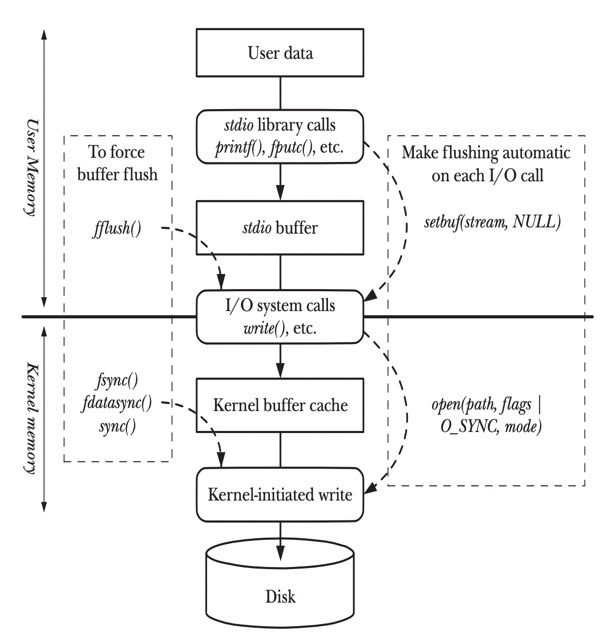
\includegraphics[scale=0.4]{unbuffio.jpeg}
\caption{Schema unbuffered I/O} 
\label{unbuffio}
\end{figure}


% Fork & Exec
\subsection{Fork \& Exec}

Prendiamo il codice di shell1.c che crea uno schell dal quale poter eseguire programmi:

\begin{lstlisting}
#include "apue.h"
#include <sys/wait.h>

int
main(void)
{
	char	buf[MAXLINE];	/* from apue.h */
	pid_t	pid;
	int		status;

	printf("%% ");	/* print prompt (printf requires %% to print %) */
	while (fgets(buf, MAXLINE, stdin) != NULL) {
		if (buf[strlen(buf) - 1] == '\n')
			buf[strlen(buf) - 1] = 0; /* replace newline with null */

		if ((pid = fork()) < 0) {
			err_sys("fork error");
		} else if (pid == 0) {		/* child */
			execlp(buf, buf, (char *)0);
			err_ret("couldn't execute: %s", buf);
			exit(127);
		}

		/* parent */
		if ((pid = waitpid(pid, &status, 0)) < 0)
			err_sys("waitpid error");
		printf("%% ");
	}
	exit(0);
}
\end{lstlisting}

avremo allora:

\begin{itemize}
	\item \hl{fgets}: funzione dello \textbf{stdoutput che legge la stringa} che dai prima di dare invio, ha come argomenti:
	
		\begin{itemize}
			\item \textbf{buf}: buffer nel quale mettere la stringa
		
			\item \textbf{MAXLINE}: proviene da una nostra libreria

\begin{lstlisting}
$ grep -rw "MAXLINE" include/
Binary file include//apue.h.gch matches
include//apue.h:#define	MAXLINE	4096			/* max line length */
\end{lstlisting}

			\item \textbf{stdin}: presente in stdiolib ed è una \textbf{struttura file che definisce uno standard input} tramite un puntatore ad un "file"
		\end{itemize}

	\item \hl{if 1}: permette di avere un null dove prima avevamo \textbackslash n
	
	\item \hl{if 2}: abbiamo una fork() che dopo che \hl{viene invocata ritorna 2 volte}, questo perché andrà a creare 2 bash identici con memorie uguali nei contenuti ma indipendenti, l'unico cambiamento è il pid. fork() andrà quindi a restituire 0 nel child e il pid del child al parent tramite getppid().

			Se pid $<$ 0 vorrà dire che la fork e fallita.
			Se pid = 0 vorrà dire che siamo nel child.
	
			Il che è molto importante dato che \hl{il codice verra' eseguito sia dal child che dal parent}, e sarà contenuto nella memora virtuale che hanno i programmi grande $2^{32}$ o $2^{64}$ in base all'OS.
	
			Appena viene eseguita l'\hl{exec, lo spazio di memoria viene azzerato} ma a discrezione del programma, vengono salvate alcune variabili di ambiente.


		\hl{execlp}: serve a far \textbf{eseguire un codice} (buf) del quale abbiamo il sorgente e l'eseguibile
	

		\hl{if 3}: serve a far andare aventi il parent.

		\hl{waitpid}: aspetta il child nel caso impieghi troppo tempo ad eseguire la sua azione, \textbf{tenendo appeso il prompt}. Con argomenti:

			\begin{itemize}
				\item \textbf{pid}: pid del child
				\item \textbf{\&status}: reindirizza l'exit code del child, quando finisce, nella variabile status
			\end{itemize}
			
\end{itemize}


\begin{figure}[H]
\centering
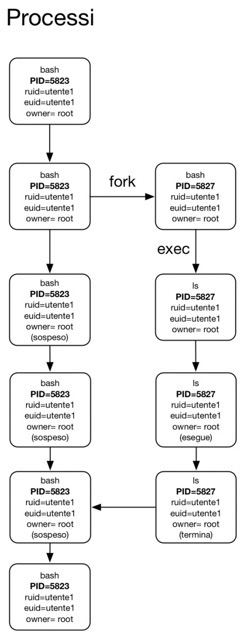
\includegraphics[scale=0.7]{fork.jpeg}
\caption{Esecuzione di fork ed exec} 
\label{fork}
\end{figure}


% Thread
\subsection{Thread}

Sono dei \hl{processi con lo stesso spazio di memoria del parent}. Per evitare che ogniuno scriva dove vuole, \hl{avviene una sincronizzazione tra le thread}. Questo metodo viene usato nelle macchine unicore per poter svolgere più operazione "contemporaneamente".

Tutto questo è \hl{orchestrato dal kernel} che gestisce il \hl{time shearing}.


% Gestione degli errori
\subsection{Gestione degli errori}

Per convenzione una funzione ritorna 0 se è andato tutto bene. Ci sono delle eccezioni, come la read, che ritorna il numero di byte letti.

Ogni valore possibile ritornato è specificato nel manuale:

\begin{lstlisting}
$ man 2 intro
...
1 EPERM Operation not permitted. An attempt was made to perform an operation limited to processes with appropriate privileges or to the owner of a file or other resources.

2 ENOENT No such file or directory. A component of a specified pathname did not exist, or the pathname was an empty string.
...
\end{lstlisting}


Per le \hl{system call}, quando avviene un errore, si \hl{avvalora la variabile "errno"} che può essere consultata in un programma con 

\begin{lstlisting}
extern int errno;
\end{lstlisting}


Con "errno" bisogna tenere in conto che:

\begin{enumerate}
	\item \hl{non viene svuotata quando passiamo l'errore}. Quindi per sapere quando è stato dato un errore bisogna andare a consultarla quando la system call viene invocata
	\item \hl{vale 0} se non usata
\end{enumerate}


Per la gestione degli errori useremo:

\begin{itemize}
	\item \hl{strerror}: restituisce la \textbf{stringa del valore} di errno
	\item \hl{perror}: legge errno e stampa un messaggio a piacere
\end{itemize}


\begin{lstlisting}
#include "apue.h"
#include <errno.h>

int
main(int argc, char *argv[])
{
	fprintf(stderr, "EACCES: %s\n", strerror(EACCES));
	errno = ENOENT;
	perror(argv[0]);
	exit(0);
}
\end{lstlisting}


dove:

\begin{itemize}
	\item \hl{fprinf}: stampa un errore allo standard specificato
\end{itemize}




\newpage
\section{Gli standard}

% Storia e basi
\subsection{Storia e basi}

La \hl{standardizzazione di UNIX e' iniziata nel 1988} facendo affidamento ad alcuni \hl{standard di C} dato che fa usi di interfaccie e prototipi.

In definitiva abbiamo gli standard:

\begin{itemize}
	\item Posix.1-2001 / SUSv3: (\url{http://pubs.opengroup.org/onlinepubs/009604599/})
	\item Posix.1-2008 / SUSv4:  più usato in ambiti di automazioni aziendali, infatti sono specializzate sullo scambio di informazione in segnali realtime. Per questo la sua certificazione non è stata presa da nessuno se non fa un IBM. (\url{http://pubs.opengroup.org/onlinepubs/9699919799/})
\end{itemize}

(\hl{PS: le versioni sono back compatibili} quindi se settiamo -D\_XOPEN\_SOURCE=700 non precludiamo la SUSv3)

Nonostante gli standard \hl{ogni OS fa delle sue modifiche su alcune cose esterne alle SUS}.

Per verificare il tipo di standard su un applicativo (\_XOPEN\_SOURCE) o un sistema (\_XOPEN\_VERSION), si fa affidamento alle "\hl{feature test macros}" consultabili dai \textbf{codici di intestazione .h}. Per esempio \_XOPEN\_SOURCE impostata a 600 o 700 indica SUSv3 o SUSv4.

\begin{lstlisting}
-D_XOPEN_SOURCE=600
\end{lstlisting}

in questo modo potremo allora andare a compilare tutti i programmi conformi su qualsiasi OS.


% Limiti
\subsection{Limiti}

Abbiamo dei limiti di compilazione che possono essere visti nei file di inestazione

runtime limit: si vedono tramite la ufnzione sysconf (es: lunghezza massima del nome dei file che dipende dal filesystem può capirlo tramite pathconf su un file qualunque di quel filesystem)

sysconf: chiamata che si può fare in qualsiasi momento e prende come argomento un name: i name argument ti restituiscono una chiave in base a cosa vuoi indagare. in pratica fanno riferimento ad un nome simbolico che si riferisce ad un valore. si fa ciò dato che questi valori potrebbero essere inseriti dnei file di include ma vicono sempre quelli di sysconf (sono precedute da \_SC\_)

pathconf: da info sul file system e per fare ciò gli serve poter arrivare ad un qualunque file del fs.

fpathconf: uguale ma dai il file descriptor

entrambe prendono un name che ha lestesse funzionalità solo è preceduto da \_PC\_




funzione path\_alloc fig 2.16 

supponendo di avere bisongo di uno sapzio dove mettere un nome di file (path) per poterlo gestire. com faccio a acapire quanto quanto spazio mi serve e quindi quanto allocarne? invece di fare un allocazione fissa ne facio una dinamica. la nostra funzione path\_alloc retiotuisce un puntatore ad una dimensione ad una memoria che può contenere il massimo di caratteri rispetto a quanto i lsistema può allocare come massima lunghezza di path. per vedere qual'è la lunghezza usaiamo la variabile limite: NAME\_MAX = 255

\begin{lstlisting}
pathconf(_PC_NAME_MAX)
\end{lstlisting}







% Definizione di un tipo

pid\_t sono definiti così dato che il progettista vuole lasciare libero il prgrammatore dal tipo 

HOMEWORK: quanto vale?

\begin{lstlisting}
$ grep -rw "pid_t" $INC | grep typedef

/sys/_types/_pid_t.h:typedef __darwin_pid_t pid_t;
/sys/_types.h:typedef __uint32_t __darwin_id_t;

$ grep -rw "__uint32_t" $INC | grep typedef

/i386/_types.h:typedef unsigned int __uint32_t;
\end{lstlisting}

tutti questi rimandi sono dati dalla \hl{portabilita'}



NUOVI CAPITOLO: file IO

in file io co sono le funzioni che fanno il buffered io che gestisce lui e si contrappone da quello dello stdlib. 

chiamata open():

1 arg: path che può essere dato come assoluto o relativo 

2: flag: sono dei bit che dicono cosa fare (es: modalità append)

notare che per le read non appena fatte le scritture il file continua a leggere da dove è stata l'ultima "posizione del file" (current posizion) della read

la prossia write sarà alla fine della read. all'inizio sta a 0 inizo file

avremo che si metterà ad 1 il bit del flag che ci serve tramite:

\begin{lstlisting}
open(file, O_RDWR | O_APPEND | O_CREAT | O_TRUNC, file_mode)
\end{lstlisting}

avremo allora: $11000001010$

con O\_RDWR: 2, O\_APPEND: 8, O\_CREAT: 512, O\_TRUNC: 1024

per lettura e scrittura invece ...



possono essere 3 argomenti quando i file lo stai creando

3. mode: privilegi con cui i file deve essere creato

openat():
si prende il file descriptor di una directory e poi passare un path che viene interpretato con un path relatico a quella directory. quidni ogni cosa viene fatta in questa orecotry anche se nelle directory a monte non si hanno i privilegi

quindi andiamo ad usare open() sulla direcory per avere il file descriptor da usare in openat()



\newpage
\section{File I/O}


% Introduzione
\subsection{Chiamata open}

I file I/O sono le \hl{funzioni che gestisce buffered I/O} ed in contrapposizione da quelle della librerira "stdlib". La chiamata open() fa parte di queste funzioni, i suoi argomenti sono:

\begin{itemize}
	\item \hl{arg}: path assoluto o relativo
	\item \hl{flag}: bit che indica l'\textbf{attivazione di alcune modalita'}. Si avrà allora a \textbf{settare il bit della flag a 1}:
	\item \hl{mode}: serve a dare i \textbf{privilegi con cui i file deve essere creato} (\textbf{da usare solo nella creazione del file})
\begin{lstlisting}
open(file, O_RDWR | O_APPEND | O_CREAT | O_TRUNC, file_mode)
\end{lstlisting}

		avremo allora: $11000001010$

		con O\_RDWR: 2, O\_APPEND: 8, O\_CREAT: 512, O\_TRUNC: 1024
		
		
\end{itemize}

Appena \hl{aperto il file questo avra' la "current position" a 0}, cioè ad inizio file. Iniziando a scrivere avremo che alla prima lettura la nostra current position si sarà spostata fino a dopo abbiamo finito di scrivere.

Per quanto riguarda \hl{read e write i bit delle flag } ....

Una variante e' \hl{openat()} che prende il file descriptor (passato dalla open() sulla directory) di una directory per passare il path relativo a quella directory. Abbiamo quindi la \hl{possibilita' di accedere a delle direcotry anceh senza avere i privilegi}. ???



\end{document}
%%%%%%%%%%%%%%%%%%%%%%%%%%%%%%%%
%%%%%% FINE DEL DOCUMENTO %%%%%%
%%%%%%%%%%%%%%%%%%%%%%%%%%%%%%%%




